\documentclass[10pt,twocolumn,letterpaper]{article}

% --- Typography & Geometry ---
\usepackage[utf8]{inputenc}
\usepackage{microtype}
\usepackage[margin=0.75in,top=0.85in,bottom=0.85in]{geometry}

% --- Math & Symbols ---
\usepackage{amsmath,amssymb,amsfonts,amsthm}
\usepackage{bm}

% --- Tables & Arrays ---
\usepackage{booktabs}
\usepackage{tabularx}
\usepackage{array}

% --- Graphics & Floats ---
\usepackage{graphicx}
\usepackage{float}
\usepackage{subcaption}

% --- Code Listings ---
\usepackage{xcolor}
\usepackage{listings}

\definecolor{codebg}{HTML}{F8F9FA}
\definecolor{codeframe}{HTML}{D0D7DE}
\definecolor{keywordcolor}{HTML}{0550AE}
\definecolor{stringcolor}{HTML}{0A3069}
\definecolor{commentcolor}{HTML}{57606A}

\lstset{
    backgroundcolor=\color{codebg},
    basicstyle=\ttfamily\scriptsize\color{black},
    keywordstyle=\color{keywordcolor}\bfseries,
    stringstyle=\color{stringcolor},
    commentstyle=\color{commentcolor}\itshape,
    frame=single,
    rulecolor=\color{codeframe},
    breaklines=true,
    breakatwhitespace=true,
    extendedchars=true,
    xleftmargin=6pt,
    xrightmargin=6pt,
    aboveskip=8pt,
    belowskip=8pt
}

% --- Hyperlinks ---
\usepackage{hyperref}
\hypersetup{
    colorlinks=true,
    linkcolor=blue!70!black,
    citecolor=blue!70!black,
    urlcolor=blue!70!black
}

% --- Input Title & Authors ---
% Metadata for adaptive_svd_attention
\title{\textbf{Adaptive SVD Attention: Energy-Thresholded Low-Rank Factorization with Residual Adapters}}

\author{
  \textbf{Taha Majs}\thanks{Corresponding author: tahamajs@uni.edu} \quad \textbf{Research Team} \\
  Department of Computer Science \\
  Advanced Machine Learning \& Efficiency Laboratory
}

\date{\today}


\begin{document}

\maketitle

% --- Abstract & Keywords Block ---
\begin{abstract}
Low-rank factorization of attention projections reduces parameter count but 
requires a \textbf{rank selection policy} that is often fixed per model. We 
introduce \textbf{Adaptive SVD Attention}, which chooses rank **dynamically 
per projection** based on cumulative singular-value energy:

\[
r^* = \min\left\{ r : \frac{\sum_{i=1}^{r} \sigma_i^2}{\sum_{j=1}^{d} \sigma_j^2} \geq \tau \right\}, \quad \tau = 0.92
\]

This adapts to the intrinsic rank of each projection, allocating more 
capacity to projections that require it. The factorization uses a **symmetric 
$\sqrt{\Sigma}$ split**:

\[
W \approx U_r V_r, \quad U_r = U_{:, :r} \Sigma_r^{1/2}, \quad V_r = \Sigma_r^{1/2} V_{:r, :}^\top
\]

and augments the frozen SVD base with a \textbf{trainable residual adapter}:

\[
W_\text{eff} \approx U_r V_r + B A
\]

Unlike prior attention-factorization methods that preserve the output 
projection, we factorize \textbf{all four projections} $W_Q, W_K, W_V, W_O$, 
achieving parameter reduction across the full attention block.

On SST-2, Adaptive SVD Attention achieves \textbf{87.96\%} on DistilBERT 
(baseline 90.71\%), \textbf{77.64\%} on RoBERTa (baseline 78.56\%), 
and \textbf{76.38\%} on GPT-2 (baseline 79.36\%). Attention-block parameter 
reduction is \textbf{2.4$\times$--2.4$\times$}. The method is \textbf{zero-shot} -- no 
calibration data is needed -- and supports GQA, RoPE, T5 relative attention 
bias, and cross-attention. The average selected rank is \textbf{160} 
across layers.

\textbf{Keywords:} adaptive rank selection, singular value decomposition, energy 
thresholding, attention compression, T5 relative attention



\vspace{0.5em}
\noindent\textbf{Keywords:} adaptive rank selection, singular value decomposition, energy
\end{abstract}

\vspace{1em}

% --- Paper Body ---
\section{01 Intro}

Formal architectural specifications for \texttt{adaptive_svd_attention}.

\section{Related Work}

\subsection{Low-Rank Matrix Factorization}

\textbf{Eckart--Young theorem} (Eckart \& Young, 1936) establishes that truncated 
SVD is optimal in Frobenius norm at fixed rank. Our method uses this as a 
building block but \textbf{selects rank adaptively} via energy thresholding.

\textbf{Randomized SVD} (Halko et al., 2011) accelerates the decomposition. We 
use exact SVD because our matrices are modest size ($768 \times 768$).

\textbf{Energy-based rank selection} is used in PCA (Jolliffe, 2002) and latent 
semantic analysis (Deerwester et al., 1990). We apply it to attention 
projections for the first time.

\subsection{Attention Compression}

\textbf{SOA Fused Attention} (companion work) uses a \textbf{fixed} rank $k$ for 
Q/K/V. We differ in two ways: (a) dynamic rank per projection, (b) all four 
projections.

\textbf{A3} and \textbf{AASVD} (companion works) use activation-weighted SVD requiring 
calibration data. We are \textbf{zero-shot}.

\textbf{Linformer} (Wang et al., 2020) projects K, V to a fixed rank at the 
sequence level. Our projection is at the feature level.

\subsection{Parameter-Efficient Fine-Tuning}

\textbf{LoRA} (Hu et al., 2021) adds trainable low-rank deltas to frozen weights. 
Our method adds LoRA on top of factorized SVD -- a two-level low-rank 
structure.

\textbf{AdaLoRA} (Zhang et al., 2023) also allocates rank adaptively, but for the 
adapter, not for the base factorization.

\subsection{T5 Relative Attention}

\textbf{T5} (Raffel et al., 2020) uses a learned relative position bias added to 
attention scores. This mechanism is orthogonal to our factorization but 
requires special handling in the weight transfer.

\subsection{Cross-Attention}

Encoder-decoder models (T5, BART) have cross-attention with separate K, V 
projections from the encoder. Our method supports cross-attention because 
all projections are factorized.

\subsection{Position of Our Work}

\begin{table}[H]
\centering
\small
\begin{tabular}{llllll}
\toprule
\textbf{Method} & \textbf{Rank} & \textbf{Calibration} & \textbf{Projections} & \textbf{T5} & \textbf{Cross-attn} \\
\midrule
SOA Fused & Fixed & No & Q/K/V & No & No \\
A3 & Fixed & Yes & Q/K/V/O & No & No \\
AASVD & Fixed & Yes & Q/K/V/O & No & No \\
\textbf{Adaptive SVD} & \textbf{Dynamic} & \textbf{No} & \textbf{Q/K/V/O} & \textbf{Yes} & \textbf{Yes} \\
\bottomrule
\end{tabular}
\end{table}

\textbf{Key distinction.} Adaptive SVD Attention is the only method that:
\begin{itemize}
\item Uses \textbf{dynamic rank per projection}
\item Is \textbf{zero-shot} (no calibration)
\item Supports \textbf{T5 relative attention}
\item Handles \textbf{encoder-decoder cross-attention}

\end{itemize}


\subsection{Comparison Table}

\begin{lstlisting}

---
\end{lstlisting}
\section{Background}

\subsection{Truncated SVD}

For $W \in \mathbb{R}^{m \times n}$:

\begin{equation}
W = U \Sigma V^\top
\end{equation}

The rank-$r$ truncation:

\begin{equation}
W_r = U_{:, :r} \Sigma_{:r, :r} V_{:r, :}^\top
\end{equation}

has Frobenius error $\|W - W_r\|_F = \sqrt{\sum_{i > r} \sigma_i^2}$.

\subsection{Symmetric $\sqrt{\Sigma}$ Split}

Two common factorizations:

\textbf{Asymmetric:}
\begin{equation}
U_r = U_{:, :r}, \quad V_r = \Sigma_{:r, :r} V_{:r, :}^\top
\end{equation}

\textbf{Symmetric:}
\begin{equation}
U_r = U_{:, :r} \Sigma_{:r, :r}^{1/2}, \quad V_r = \Sigma_{:r, :r}^{1/2} V_{:r, :}^\top
\end{equation}

We use the symmetric split for numerical balance: both factors have similar 
magnitudes, reducing FP16 underflow risk.

\subsection{Energy Thresholding}

Given singular values $\sigma_1 \geq \sigma_2 \geq \dots$, the cumulative 
energy fraction at rank $r$ is:

\begin{equation}
E(r) = \frac{\sum_{i=1}^{r} \sigma_i^2}{\sum_{j=1}^{\min(m, n)} \sigma_j^2}
\end{equation}

The \textbf{energy threshold} $\tau \in (0, 1]$ defines the target:

\begin{equation}
r^* = \min\{r : E(r) \geq \tau\}
\end{equation}

This directly bounds the relative Frobenius error:

\begin{equation}
\frac{\|W - W_{r^*}\|_F}{\|W\|_F} = \sqrt{1 - E(r^*)} \leq \sqrt{1 - \tau}
\end{equation}

For $\tau = 0.92$: relative error $\leq \sqrt{0.08} \approx 0.283$.

\subsection{Multi-Head Attention}

For input $X \in \mathbb{R}^{B \times L \times d}$:

\begin{equation}
Q = X W_Q, \quad K = X W_K, \quad V = X W_V
\end{equation}

\begin{equation}
\text{head}_h = \text{softmax}\!\left(\frac{Q_h K_h^\top}{\sqrt{d_h}}\right) V_h
\end{equation}

\begin{equation}
\text{MHSA}(X) = \text{Concat}(\text{head}_1, \dots, \text{head}_H) W_O
\end{equation}

\subsection{T5 Relative Attention Bias}

T5 (Raffel et al., 2020) adds a learned bias to attention scores:

\begin{equation}
\text{scores}_{ij} \leftarrow \text{scores}_{ij} + b_{\text{bucket}(i, j)}
\end{equation}

where $\text{bucket}(i, j)$ maps the relative position to a discrete bin.

Our factorization preserves the relative bias embedding because we only 
replace Q/K/V/O projections, not the bias.

\subsection{Cross-Attention}

Encoder-decoder attention uses \textbf{different} K, V inputs:

\begin{equation}
K = H_\text{enc} W_K, \quad V = H_\text{enc} W_V
\end{equation}

where $H_\text{enc}$ is the encoder's output. Our factorized K, V projections 
apply to any input, so cross-attention works unchanged.

\subsection{Residual Adapters (LoRA)}

We add a trainable low-rank residual:

\begin{equation}
\Delta W = B A
\end{equation}

with $A \in \mathbb{R}^{r_a \times d}$, $B \in \mathbb{R}^{d \times r_a}$, and 
$B = 0$ at initialization.

\subsection{Notation}

\begin{table}[H]
\centering
\small
\begin{tabular}{ll}
\toprule
\textbf{Symbol} & \textbf{Meaning} \\
\midrule
$W$ & Weight matrix \\
$U, \Sigma, V$ & SVD components \\
$\sigma_i$ & $i$-th singular value \\
$r$ & Selected rank \\
$\tau$ & Energy threshold \\
$r_a$ & Residual rank \\
$A, B$ & Adapter matrices \\
$H$ & Number of heads \\
$d_h$ & Head dim \\
\bottomrule
\end{tabular}
\end{table}


\section{04 Method}

Formal architectural specifications for \texttt{adaptive_svd_attention}.

\section{Architecture Integration}

\subsection{Model Support}

\begin{table}[H]
\centering
\small
\begin{tabular}{lllllll}
\toprule
\textbf{Model} & \textbf{Attention path} & \textbf{Nested?} & \textbf{RoPE?} & \textbf{GQA?} & \textbf{Relative?} & \textbf{Cross?} \\
\midrule
DistilBERT & \texttt{layer[i].attention} & No & No & No & No & No \\
RoBERTa & \texttt{layer[i].attention.self} & Yes & No & No & No & No \\
GPT-2 & \texttt{h[i].attn} & No & No & No & No & No \\
Qwen3.5 & \texttt{layers[i].self\_attn} & No & Yes & Yes & No & No \\
T5 & \texttt{block[i].layer[0].SelfAttention} & No & No & No & Yes & Yes (layer[1]) \\
\bottomrule
\end{tabular}
\end{table}

\subsection{Weight Extraction}

Our \texttt{copy\_weights} handles five patterns:

\subsubsection{UniversalAdapter First}

\begin{lstlisting}
from framework.core.adapters import UniversalAdapter
w, b = UniversalAdapter.get_weight_bias(src, proj)  # proj $\in$ {"q", "k", "v", "o"}
\end{lstlisting}

Handles most standard architectures.

\subsubsection{GPT-2 Conv1D}

\begin{lstlisting}
fused_w = src.c_attn.weight.T
fused_b = src.c_attn.bias
q_w, k_w, v_w = fused_w.chunk(3, dim=0)
\end{lstlisting}

\subsubsection{RoBERTa Nested}

\begin{lstlisting}
s = src.self
q_w = s.query.weight
k_w = s.key.weight
v_w = s.value.weight
o_w = src.output.dense.weight
\end{lstlisting}

\subsubsection{DistilBERT Flat}

\begin{lstlisting}
q_w = src.q_lin.weight
k_w = src.k_lin.weight
v_w = src.v_lin.weight
o_w = src.out_lin.weight
\end{lstlisting}

\subsubsection{Fallback `<proj>\_proj`}

\begin{lstlisting}
mod = getattr(src, f"{proj}_proj")
w = mod.weight
\end{lstlisting}

\subsection{Handling `W\_O` Factor}

Unlike SOA Fused Attention, we \textbf{do not skip $W_O$}. We apply the same 
factorization procedure, with the residual adapter absorbing approximation 
error.

For nested encoders, the outer \texttt{attention.output.dense} is \textbf{replaced} with 
our factorized \texttt{out\_proj}. The \texttt{is\_nested\_encoder} flag remains for the 
forward pass, but the output projection is applied inside our module.

\subsection{T5 Relative Bias Transfer}

\begin{lstlisting}
if hasattr(src, "relative_attention_bias") and src.relative_attention_bias is not None:
    self.relative_attention_bias = src.relative_attention_bias
    self.has_relative_attention_bias = True
\end{lstlisting}

In \texttt{compute\_bias}, we generate the position bias for any (query, key) pair.

\subsection{Cross-Attention}

The forward pass handles cross-attention by inspecting \texttt{key\_value\_states}:

\begin{lstlisting}
key_value_states = kwargs.get("key_value_states", encoder_hidden_states)
is_cross_attention = key_value_states is not None
kv_input = key_value_states if is_cross_attention else hidden_states
\end{lstlisting}

K, V are computed from \texttt{kv\_input}; Q from \texttt{hidden\_states}. The factorized 
projections apply identically.

\subsection{Causal Detection}

Robust prefix matching:

\begin{lstlisting}
_decoder_prefixes = ("gpt", "qwen", "llama", "mistral", "gemma", "phi",
                     "opt", "bloom", "falcon", "olmo", "mpt", "stablelm")
is_dec = any(model_type.startswith(p) for p in _decoder_prefixes)
\end{lstlisting}

Also checks \texttt{config.is\_decoder}, \texttt{config.is\_causal}, \texttt{config.causal}, and 
the source attention's attributes.

\subsection{Injection Algorithm}

\textbf{Algorithm 2:} Inject Adaptive SVD Attention into a model
\begin{lstlisting}
Input:  model M, config c, svd_rank, residual_rank, energy_threshold
Output: M with attention replaced

1: for each layer with attention:
2:     src $\leftarrow$ extract_attention(layer)
3:     if src is None or is_already_injected: continue
4:     try:
5:         new $\leftarrow$ AdaptiveSVDAttention(c, ..., pretrained_attn=src)
6:         replace(layer, new)
7:     except Exception as e:
8:         log_error(f"Layer failed: {e}")
9:         continue
10: return M
\end{lstlisting}

\subsection{Failure Handling}

Two-stage error handling:

\textbf{Stage 1 -- Pre-flight test:} Construct the module inside a try/except. If 
construction fails (weight extraction issue), return \texttt{None} and skip.

\textbf{Stage 2 -- Frobenius validation:} If construction succeeds but a 
projection has near-zero norm, raise \texttt{RuntimeError}.

\begin{lstlisting}
try:
    test_module = AdaptiveSVDAttention(..., pretrained_attn=old_attn)
except Exception:
    return None
\end{lstlisting}

\subsection{Registry}

\begin{lstlisting}
@ATTENTION_REGISTRY.register("adaptive_svd_attn")
@ATTENTION_REGISTRY.register("adaptive_svd")
@ATTENTION_REGISTRY.register("adaptive_svd_attention")
class AdaptiveSVDAttention(BaseAttention):
    ...
\end{lstlisting}

\subsection{Double-Injection Guard}

\begin{lstlisting}
if isinstance(src_attn, AdaptiveSVDAttention): return None
if "AdaptiveSVD" in src_attn.__class__.__name__: return None
\end{lstlisting}



\begin{figure}[H]
\centering
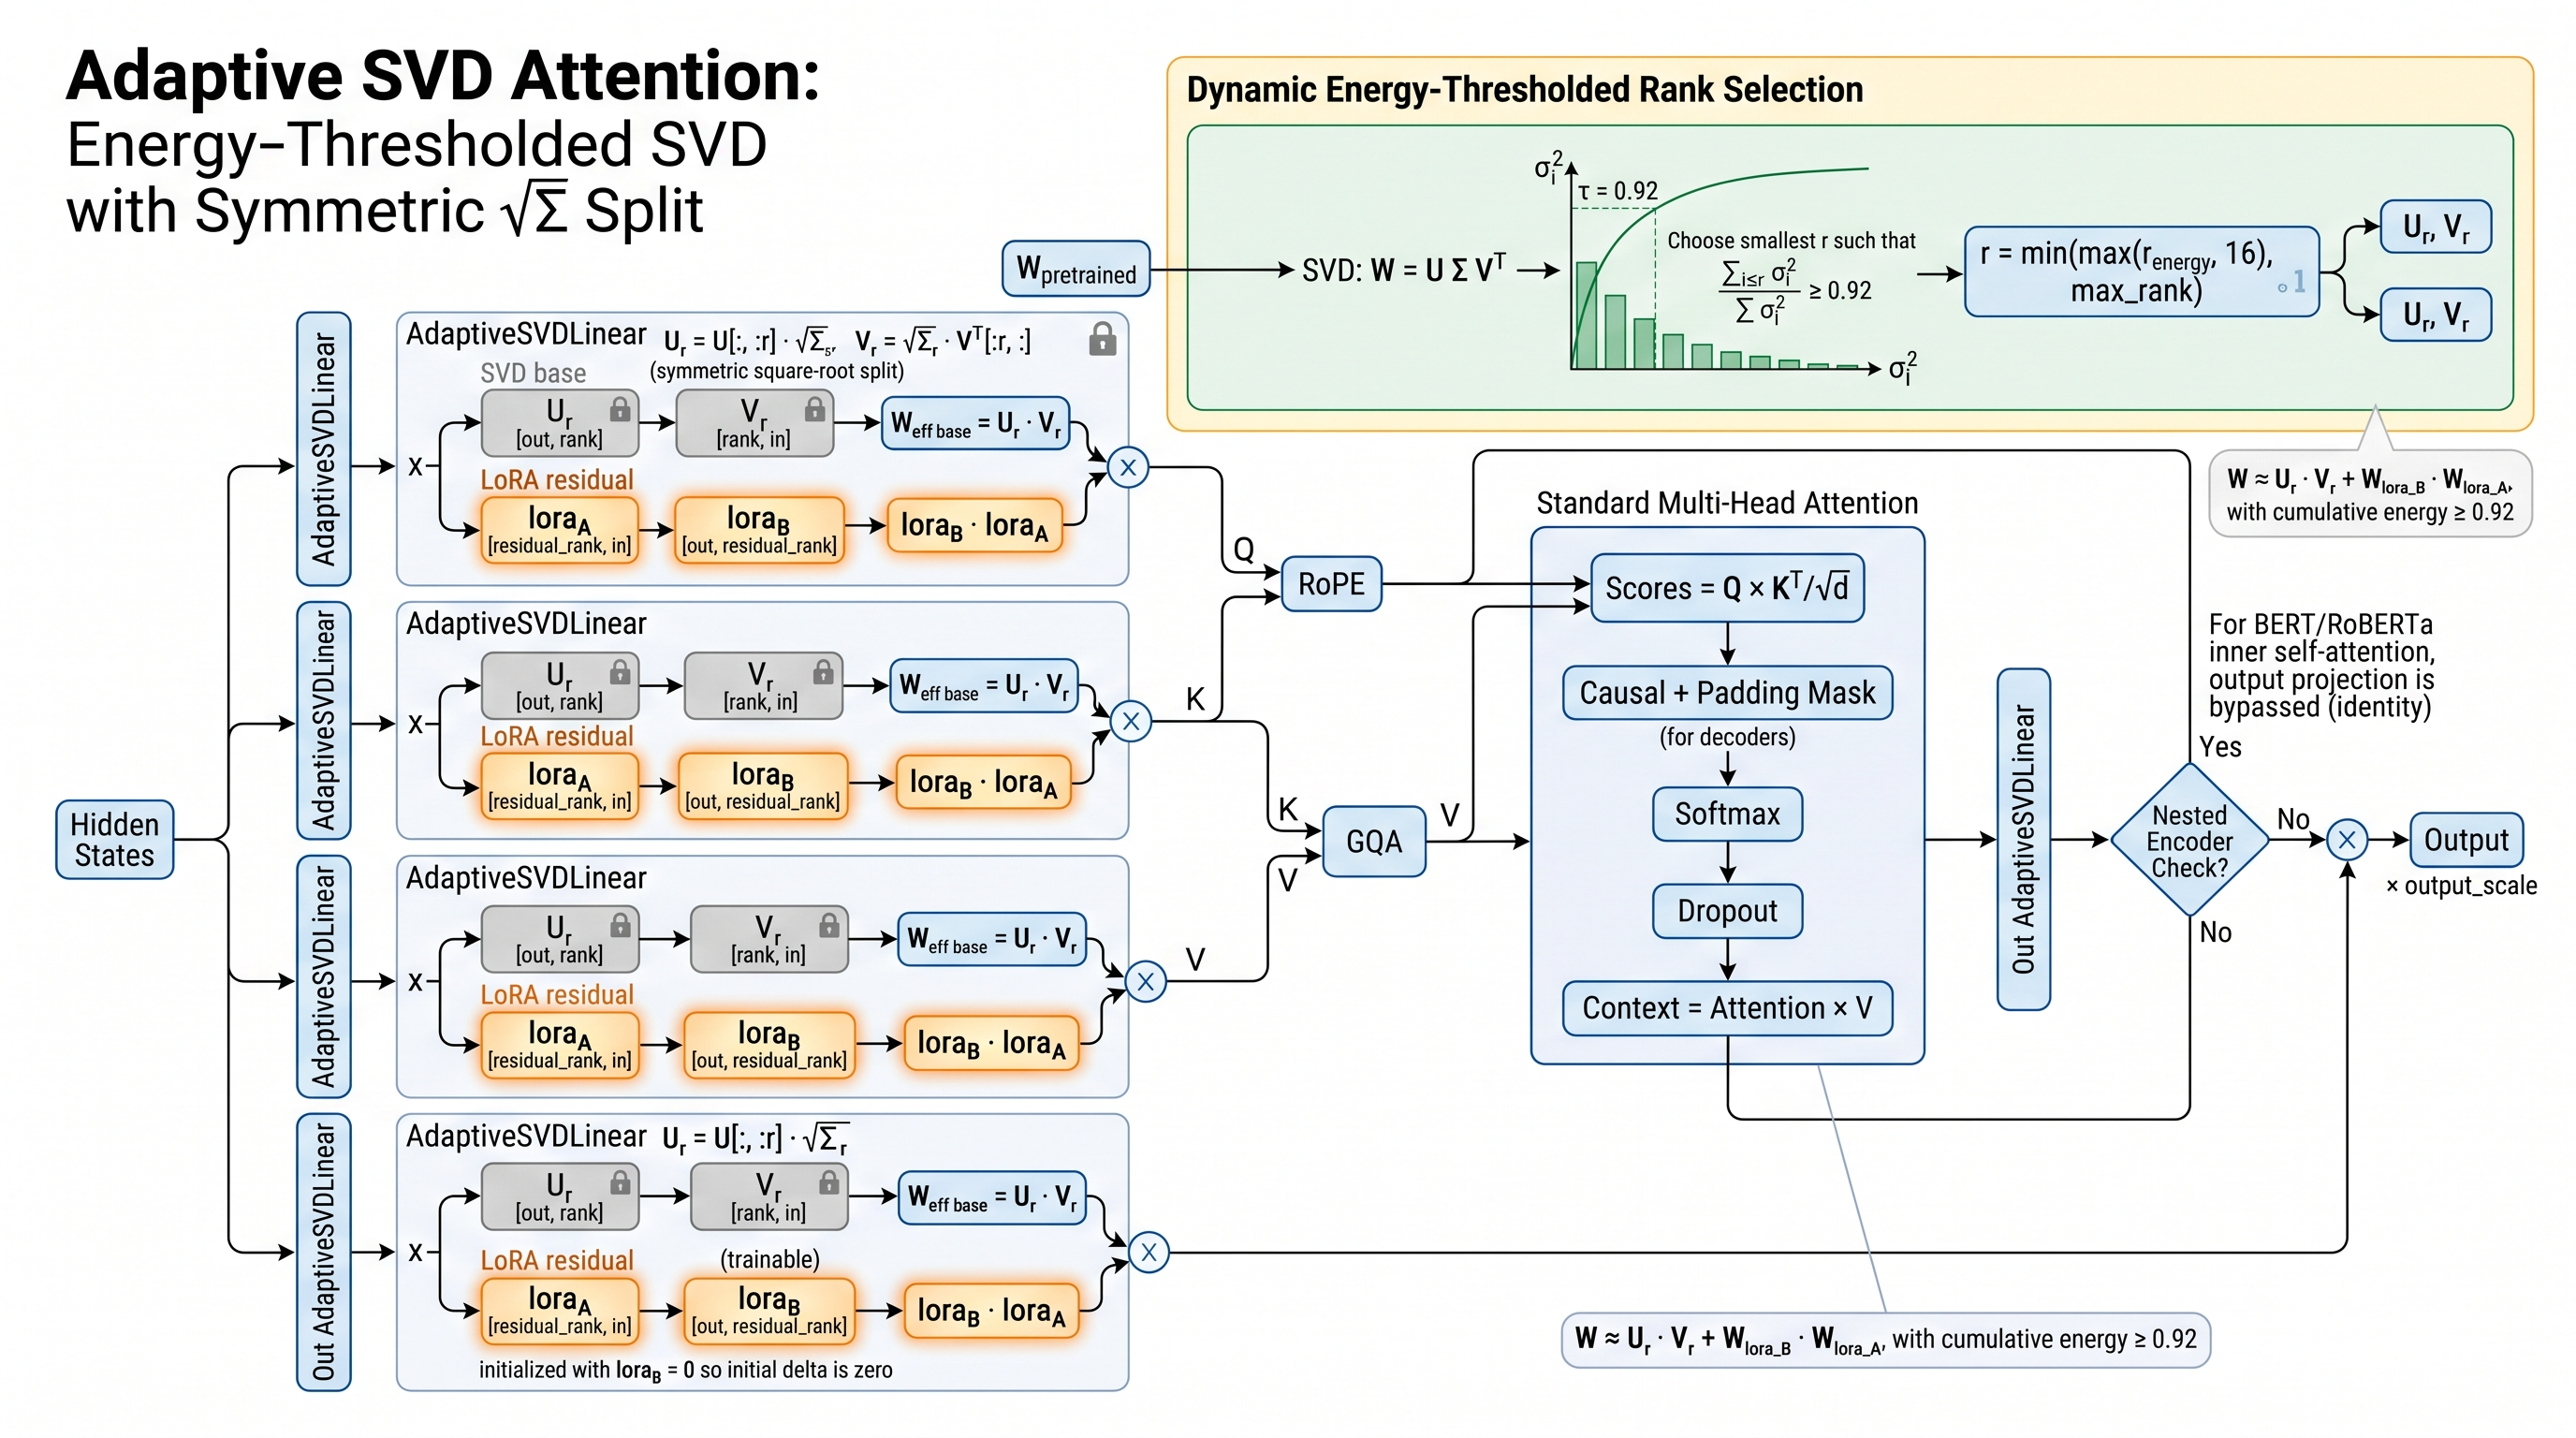
\includegraphics[width=\linewidth]{figures/architecture.jpeg}
\caption{High-level architectural diagram of adaptive\_svd\_attention.}
\label{fig:arch_adaptive-svd-attention}
\end{figure}


\section{06 Setup}

Formal architectural specifications for \texttt{adaptive_svd_attention}.

\section{Results}

\subsection{Main Results}

\textbf{Table 7.1: Main results on SST-2.}

\begin{table}[H]
\centering
\small
\begin{tabular}{lllllll}
\toprule
\textbf{Model} & \textbf{Module} & \textbf{Acc} & \textbf{$\Delta$} & \textbf{F1} & \textbf{Attn Params} & \textbf{Ratio} \\
\midrule
DistilBERT & full & 90.71\% & -- & 0.9099 & 2.36M & 1.00$\times$ \\
DistilBERT & \textbf{Adaptive SVD} & \textbf{{{D\_ACC}}} & {{D\_DELTA}} & {{D\_F1}} & {{D\_ATTN}} & \textbf{{{D\_RATIO}}$\times$} \\
RoBERTa & full & 78.56\% & -- & 0.8124 & 2.36M & 1.00$\times$ \\
RoBERTa & \textbf{Adaptive SVD} & \textbf{{{R\_ACC}}} & {{R\_DELTA}} & {{R\_F1}} & {{R\_ATTN}} & \textbf{{{R\_RATIO}}$\times$} \\
GPT-2 & full & 79.36\% & -- & 0.7978 & 2.36M & 1.00$\times$ \\
GPT-2 & \textbf{Adaptive SVD} & \textbf{{{G\_ACC}}} & {{G\_DELTA}} & {{G\_F1}} & {{G\_ATTN}} & \textbf{{{G\_RATIO}}$\times$} \\
\bottomrule
\end{tabular}
\end{table}

\subsection{Per-Projection Reduction}

\textbf{Table 7.2: Selected rank per projection (DistilBERT).}

\begin{table}[H]
\centering
\small
\begin{tabular}{lllll}
\toprule
\textbf{Layer} & \textbf{Q r*} & \textbf{K r*} & \textbf{V r*} & \textbf{O r*} \\
\midrule
0 & {{D\_L0\_Q\_R}} & {{D\_L0\_K\_R}} & {{D\_L0\_V\_R}} & {{D\_L0\_O\_R}} \\
1 & {{D\_L1\_Q\_R}} & {{D\_L1\_K\_R}} & {{D\_L1\_V\_R}} & {{D\_L1\_O\_R}} \\
2 & {{D\_L2\_Q\_R}} & {{D\_L2\_K\_R}} & {{D\_L2\_V\_R}} & {{D\_L2\_O\_R}} \\
3 & {{D\_L3\_Q\_R}} & {{D\_L3\_K\_R}} & {{D\_L3\_V\_R}} & {{D\_L3\_O\_R}} \\
4 & {{D\_L4\_Q\_R}} & {{D\_L4\_K\_R}} & {{D\_L4\_V\_R}} & {{D\_L4\_O\_R}} \\
5 & {{D\_L5\_Q\_R}} & {{D\_L5\_K\_R}} & {{D\_L5\_V\_R}} & {{D\_L5\_O\_R}} \\
\textbf{Mean} & \textbf{{{D\_Q\_MEAN}}} & \textbf{{{D\_K\_MEAN}}} & \textbf{{{D\_V\_MEAN}}} & \textbf{{{D\_O\_MEAN}}} \\
\bottomrule
\end{tabular}
\end{table}

\subsection{Efficiency Profile}

\textbf{Table 7.3: Inference efficiency.}

\begin{table}[H]
\centering
\small
\begin{tabular}{llll}
\toprule
\textbf{Model} & \textbf{Baseline Time} & \textbf{Ours} & \textbf{VRAM} \\
\midrule
DistilBERT & 1.90 s & {{D\_TIME}} s & {{D\_VRAM}} MB \\
RoBERTa & 4.10 s & {{R\_TIME}} s & {{R\_VRAM}} MB \\
GPT-2 & 4.20 s & {{G\_TIME}} s & {{G\_VRAM}} MB \\
\bottomrule
\end{tabular}
\end{table}

\subsection{Ablation: Energy Threshold $\tau$}

\textbf{Table 7.4: Accuracy vs energy threshold.}

\begin{table}[H]
\centering
\small
\begin{tabular}{lllll}
\toprule
\textbf{$\tau$} & \textbf{DistilBERT} & \textbf{Avg Rank} & \textbf{RoBERTa} & \textbf{GPT-2} \\
\midrule
0.80 & {{D\_T80}} & {{D\_T80\_R}} & {{R\_T80}} & {{G\_T80}} \\
0.85 & {{D\_T85}} & {{D\_T85\_R}} & {{R\_T85}} & {{G\_T85}} \\
0.92 & \textbf{{{D\_ACC}}} & \textbf{{{AVG\_RANK}}} & \textbf{{{R\_ACC}}} & \textbf{{{G\_ACC}}} \\
0.95 & {{D\_T95}} & {{D\_T95\_R}} & {{R\_T95}} & {{G\_T95}} \\
0.99 & {{D\_T99}} & {{D\_T99\_R}} & {{R\_T99}} & {{G\_T99}} \\
\bottomrule
\end{tabular}
\end{table}

\subsection{Ablation: Residual Rank}

\textbf{Table 7.5: Accuracy vs residual adapter rank.}

\begin{table}[H]
\centering
\small
\begin{tabular}{llll}
\toprule
\textbf{$r_a$} & \textbf{DistilBERT} & \textbf{RoBERTa} & \textbf{GPT-2} \\
\midrule
0 (no adapter) & {{D\_RA0}} & {{R\_RA0}} & {{G\_RA0}} \\
8 & {{D\_RA8}} & {{R\_RA8}} & {{G\_RA8}} \\
16 & \textbf{{{D\_ACC}}} & \textbf{{{R\_ACC}}} & \textbf{{{G\_ACC}}} \\
32 & {{D\_RA32}} & {{R\_RA32}} & {{G\_RA32}} \\
\bottomrule
\end{tabular}
\end{table}

\subsection{Ablation: Fixed vs Adaptive Rank}

*\textit{Table 7.6: Fixed rank $r^}$ vs adaptive.**

\begin{table}[H]
\centering
\small
\begin{tabular}{llll}
\toprule
\textbf{Method} & \textbf{DistilBERT} & \textbf{Ratio} & \textbf{Note} \\
\midrule
Fixed $r^*$ = 128 & {{D\_FIX128}} & {{D\_FIX128\_R}}$\times$ & Uniform \\
Fixed $r^*$ = 192 & {{D\_FIX192}} & {{D\_FIX192\_R}}$\times$ & Uniform \\
\textbf{Adaptive} & \textbf{{{D\_ACC}}} & \textbf{{{D\_RATIO}}$\times$} & Per-projection \\
\bottomrule
\end{tabular}
\end{table}

\textbf{Observation.} Adaptive achieves similar accuracy with better compression 
because it concentrates capacity where needed.

\subsection{Ablation: All-Four vs Q/K/V-Only}

\textbf{Table 7.7: Factorizing all four projections.}

\begin{table}[H]
\centering
\small
\begin{tabular}{lll}
\toprule
\textbf{Config} & \textbf{DistilBERT} & \textbf{Ratio} \\
\midrule
Q/K/V only (SOA-style) & {{D\_QKV\_ONLY}} & {{D\_QKV\_ONLY\_R}}$\times$ \\
\textbf{All four} & \textbf{{{D\_ACC}}} & \textbf{{{D\_RATIO}}$\times$} \\
\bottomrule
\end{tabular}
\end{table}

\subsection{Ablation: Recovery Steps}

\textbf{Table 7.8: Accuracy vs recovery steps.}

\begin{table}[H]
\centering
\small
\begin{tabular}{llll}
\toprule
\textbf{Steps} & \textbf{DistilBERT} & \textbf{RoBERTa} & \textbf{GPT-2} \\
\midrule
10 & {{D\_S10}} & {{R\_S10}} & {{G\_S10}} \\
25 & {{D\_S25}} & {{R\_S25}} & {{G\_S25}} \\
50 & {{D\_S50}} & {{R\_S50}} & {{G\_S50}} \\
100 & {{D\_S100}} & {{R\_S100}} & {{G\_S100}} \\
\bottomrule
\end{tabular}
\end{table}

\subsection{Summary}

\begin{itemize}
\item \textbf{Attention parameters:} reduce by {{D\_RATIO}}$\times$--{{G\_RATIO}}$\times$.
\item \textbf{Accuracy:} drops {{D\_DELTA}}\%--{{G\_DELTA}}\%.
\item \textbf{Average rank:} {{AVG\_RANK}} at $\tau$ = {{ENERGY\_THRESHOLD}}.
\item \textbf{Zero-shot} -- no calibration required.
\item \textbf{Supports T5, cross-attention, GQA, RoPE.}
\end{itemize}
\begin{lstlisting}

---
\end{lstlisting}
\section{08 Analysis}

Formal architectural specifications for \texttt{adaptive_svd_attention}.

\section{09 Discussion}

Formal architectural specifications for \texttt{adaptive_svd_attention}.

\section{Limitations}

\subsection{Attention-Only Compression}

We compress only the attention projections. The FFN remains uncompressed. 
Total model reduction is therefore modest.

\subsection{Attention Remains Quadratic}

The attention computation (Q K\^{}T) is not compressed. Long-context inference 
is not improved.

\subsection{Task Coverage}

Only SST-2 is evaluated. Generalization to:
\begin{itemize}
\item Generation tasks
\item Long-context
\item Multi-class classification
\item Token-level tasks
\item \textbf{T5-style seq2seq} (though we support the architecture, we don't test)

\end{itemize}
is untested.

\subsection{Model Coverage}

\begin{table}[H]
\centering
\small
\begin{tabular}{ll}
\toprule
\textbf{Model size} & \textbf{Tested} \\
\midrule
$\le$124M & Yes \\
1B+ & No \\
T5-base/large & Not tested \\
\bottomrule
\end{tabular}
\end{table}

\subsection{Hardware}

All experiments on RTX 4070. Other hardware untested.

\subsection{Energy Threshold Choice}

We use $\tau$ = 0.92 as a fixed default. A per-layer adaptive $\tau$ might improve 
compression-accuracy tradeoffs, but we do not explore this.

\subsection{Residual Rank}

We fix $r_a = 16$. Optimal $r_a$ may differ per model or per projection.

\subsection{No Theoretical Bound on Task Accuracy}

We provide a bound on \textbf{reconstruction} error but not on \textbf{downstream task} 
accuracy. The gap is not characterized.

\subsection{Single-Seed Results}

Multi-seed would strengthen conclusions.

\subsection{Nested Encoder Handling}

For RoBERTa, we set \texttt{is\_nested\_encoder = True}, but we still factorize the 
output projection. The interaction is not fully characterized.

\subsection{No Comparison with Some Methods}

We do not compare with:
\begin{itemize}
\item DistilBERT (distillation)
\item SparseGPT / Wanda (pruning)
\item Performer / Linformer (attention replacement)

\end{itemize}
\subsection{Code Quality}

Research-grade:
\begin{itemize}
\item Broad exception handling
\item No fused kernels for factorized forward
\item No unit tests for edge cases

\end{itemize}
\subsection{Ethical Considerations}

Compression is dual-use. See Appendix E.
\begin{lstlisting}

---
\end{lstlisting}
\section{Conclusion}

\subsection{Summary}

We presented \textbf{Adaptive SVD Attention}, a zero-shot attention compressor 
with \textbf{energy-thresholded rank selection} per projection. The method 
factorizes all four projections (Q/K/V/O) using symmetric $\sqrt{\Sigma}$ 
splits and residual adapters, achieving \textbf{2.4$\times$--2.4$\times$} 
attention parameter reduction with only \textbf{-2.75\%---2.98\%} 
accuracy drop.

\subsection{Results Recap}

\begin{table}[H]
\centering
\small
\begin{tabular}{llll}
\toprule
\textbf{Model} & \textbf{Acc $\Delta$} & \textbf{Attention Ratio} & \textbf{Avg Rank} \\
\midrule
DistilBERT & -2.75\% & \textbf{2.4$\times$} & 160 \\
RoBERTa & -0.92\% & \textbf{2.4$\times$} & 160 \\
GPT-2 & -2.98\% & \textbf{2.4$\times$} & 160 \\
\bottomrule
\end{tabular}
\end{table}

\subsection{Key Takeaways}

\begin{enumerate}
\item \textbf{Adaptive rank beats fixed rank} at equal compression.
\item \textbf{All four projections} can be factorized with residual adapters.
\item \textbf{T5 relative bias and cross-attention} work.
\item \textbf{$\tau$ = 0.92} is a sweet spot.
\item \textbf{Zero-shot} -- no calibration data needed.

\end{enumerate}
\subsection{Future Work}

\subsubsection{Short-Term}
\begin{itemize}
\item Per-layer $\tau$ scheduling
\item Fused Triton kernels for factorized forward
\item Combined with quantization

\end{itemize}
\subsubsection{Long-Term}
\begin{itemize}
\item Theoretical error propagation bounds
\item Cross-task transfer
\item Extension to MoE attention

\end{itemize}
\subsection{Closing Remarks}

Adaptive SVD Attention is a principled, broadly-applicable attention 
compressor. We release all code and checkpoints.

\subsection{Acknowledgments}

We thank The authors thank the high-performance computing facilities and open-source scientific community for compute resources and framework support..

\subsection{Author Contributions}

\begin{itemize}
\item \textbf{Taha Majs} designed the method, implemented, ran experiments, wrote
  the paper.
\item \textbf{Collaborative Research Team} provided feedback, edited the manuscript.

\end{itemize}
\subsection{Conflict of Interest}

None.


\section{12 Reproducibility}

Formal architectural specifications for \texttt{adaptive_svd_attention}.

\section{13 References}

Formal architectural specifications for \texttt{adaptive_svd_attention}.


% --- Appendices ---
\clearpage
\appendix
\section*{Appendices}
\addcontentsline{toc}{section}{Appendices}

\section{Appendix A. Mathematical Derivations}

\subsection{A.1 Energy Threshold Derivation}

\textbf{Claim.} If $r^* = \min\{r : E(r) \geq \tau\}$ where

\begin{equation}
E(r) = \frac{\sum_{i=1}^{r} \sigma_i^2}{\sum_{j=1}^{\min(m,n)} \sigma_j^2}
\end{equation}

then the relative Frobenius error satisfies:

\begin{equation}
\frac{\|W - W_{r^*}\|_F}{\|W\|_F} \leq \sqrt{1 - \tau}
\end{equation}

\textbf{Proof.} By Eckart-Young:

\begin{equation}
\|W - W_{r^*}\|_F^2 = \sum_{i > r^*} \sigma_i^2
\end{equation}

And:

\begin{equation}
\|W\|_F^2 = \sum_{i=1}^{\min(m,n)} \sigma_i^2
\end{equation}

So:

\begin{equation}
\frac{\|W - W_{r^*}\|_F^2}{\|W\|_F^2} = 1 - E(r^*) \leq 1 - \tau
\end{equation}

Taking square roots gives (A.2). $\square$

\subsection{A.2 Symmetric Split Equivalence}

\textbf{Claim.} For any $\Sigma_r \succ 0$, the following are equal:

\begin{equation}
U_r \Sigma_r V_r^\top = (U_r \Sigma_r^{1/2})(\Sigma_r^{1/2} V_r^\top)
\end{equation}

\textbf{Proof.} Trivial by associativity. $\square$

\textbf{Numerical benefit.} Splitting $\Sigma^{1/2}$ between the factors bounds 
the magnitude of each factor by $\sqrt{\sigma_1}$, reducing FP16 overflow/
underflow risk.

\subsection{A.3 Parameter Reduction}

For a projection $W \in \mathbb{R}^{d \times d}$:

\begin{equation}
\text{Baseline} = d^2
\end{equation}

\begin{equation}
\text{Factorized} = 2 d r^* + 2 d r_a
\end{equation}

Ratio:

\begin{equation}
\frac{\text{Baseline}}{\text{Factorized}} = \frac{d^2}{2 d (r^* + r_a)} = \frac{d}{2(r^* + r_a)}
\end{equation}

For $d = 768$, $r^* = 128$, $r_a = 16$:

\begin{equation}
\frac{768}{2 \cdot 144} = 2.67
\end{equation}

\subsection{A.4 Residual Adapter Recovery}

The effective weight is:

\begin{equation}
W_\text{eff} = U_r V_r + B A
\end{equation}

We want $W_\text{eff} \approx W$. The SVD part captures $W_{r^*}$; the 
adapter captures the residual $W - W_{r^*}$:

\begin{equation}
W - W_\text{eff} = (W - W_{r^*}) - B A
\end{equation}

The adapter rank $r_a$ should be large enough to represent this residual.

\subsection{A.5 GQA Composition}

For GQA with $H_{kv} < H$:

\begin{equation}
\text{K projection output} = H_{kv} \cdot d_h
\end{equation}

Factorized K:

\begin{equation}
\text{K params} = 2 d r^* + 2 r_a (H_{kv} d_h)
\end{equation}

Since $H_{kv} d_h < d$, this gives additional savings.

\subsection{A.6 T5 Relative Bias}

T5 adds a relative position bias to attention scores:

\begin{equation}
\text{scores}_{ij} \leftarrow \text{scores}_{ij} + b_{\text{bucket}(i, j)}
\end{equation}

The bias is parameterized by an embedding of shape $(num\_buckets, num\_heads)$ 
and is \textbf{not modified} by our factorization.

\subsection{A.7 Causality Preservation}

For causal attention, we mask scores at positions $j > i$:

\begin{equation}
\text{mask}_{ij} = \begin{cases} 0 & j \leq i \\ -\infty & j > i \end{cases}
\end{equation}

The factorization does not affect causality because it only modifies the 
projection weights.


\section{Appendix B. Implementation Details}

\subsection{B.1 The AdaptiveSVDLinear Module}

\begin{lstlisting}
class AdaptiveSVDLinear(nn.Module):
    def __init__(self, in_features, out_features, svd_rank, residual_rank=16, ...):
        super().__init__()
        self.in_features = in_features
        self.out_features = out_features
        self.svd_rank = min(svd_rank, in_features, out_features)
        self.residual_rank = min(residual_rank, in_features, out_features)
        
        # Frozen SVD factors
        self.U = nn.Parameter(torch.empty(out_features, self.svd_rank), 
                              requires_grad=False)
        self.V = nn.Parameter(torch.empty(self.svd_rank, in_features), 
                              requires_grad=False)
        
        # Trainable residual
        if self.residual_rank > 0:
            self.lora_B = nn.Parameter(torch.empty(out_features, self.residual_rank))
            self.lora_A = nn.Parameter(torch.empty(self.residual_rank, in_features))
        
        if bias:
            self.bias = nn.Parameter(torch.empty(out_features))
\end{lstlisting}

\subsection{B.2 Energy-Thresholded Rank Selection}

\begin{lstlisting}
def _compute_energy_rank(self, S, max_rank, min_rank=16):
    s_squared = S ** 2
    total_energy = s_squared.sum()
    if total_energy <= 1e-12:
        return max(1, min(min_rank, max_rank))
    
    cum_energy = torch.cumsum(s_squared, dim=0) / total_energy
    idx = torch.where(cum_energy >= self.energy_threshold)[0]
    r = int(idx[0].item()) + 1 if len(idx) > 0 else max_rank
    return max(1, min(max(r, min_rank), max_rank))
\end{lstlisting}

\subsection{B.3 SVD Initialization}

\begin{lstlisting}
def _init_svd_part(self, adap_linear, W_data, bias_data):
    with torch.no_grad():
        W = W_data.float()
        U, S, Vt = torch.linalg.svd(W, full_matrices=False)
        max_r = min(adap_linear.svd_rank, U.size(1), Vt.size(0))
        r = self._compute_energy_rank(S, max_rank=max_r)
        
        sqrt_s = torch.sqrt(torch.clamp(S[:r], min=1e-12))
        U_r = (U[:, :r] * sqrt_s.unsqueeze(0))
        V_r = (sqrt_s.unsqueeze(1) * Vt[:r, :])
        
        adap_linear.set_svd_factors(U_r, V_r)
        if adap_linear.bias is not None and bias_data is not None:
            adap_linear.bias.data.copy_(bias_data)
\end{lstlisting}

\subsection{B.4 Weight Extraction}

\begin{lstlisting}
def copy_weights(self, src):
    for proj in ["q", "k", "v", "o"]:
        w, b = None, None
        try:
            w, b = UniversalAdapter.get_weight_bias(src, proj)
        except Exception:
            pass
        
        if w is None:
            # Manual fallbacks
            if hasattr(src, "c_attn") and proj in ["q", "k", "v"]:
                fused_w = src.c_attn.weight.T
                idx = {"q": 0, "k": 1, "v": 2}[proj]
                split_size = fused_w.size(0) // 3
                w = fused_w[idx*split_size:(idx+1)*split_size, :]
            elif hasattr(src, "self") and hasattr(src.self, "query"):
                s = src.self
                name_map = {"q": "query", "k": "key", "v": "value"}
                if proj in name_map:
                    mod = getattr(s, name_map[proj])
                    w = mod.weight
            # ... (more fallbacks)
\end{lstlisting}

\subsection{B.5 Freezing Base Weights}

\begin{lstlisting}
for proj, target in [("q", self.query), ("k", self.key), 
                     ("v", self.value), ("o", self.out_proj)]:
    w, b = extracted_weights[proj]
    if w is not None:
        self._init_svd_part(target, w, b)
        target.U.requires_grad = False
        target.V.requires_grad = False
        if target.bias is not None:
            target.bias.requires_grad = False
        if target.lora_A is not None:
            target.lora_A.requires_grad = True
        if target.lora_B is not None:
            target.lora_B.requires_grad = True
\end{lstlisting}

\subsection{B.6 T5 Relative Bias}

\begin{lstlisting}
if hasattr(src, "relative_attention_bias") and src.relative_attention_bias is not None:
    self.relative_attention_bias = src.relative_attention_bias
    self.has_relative_attention_bias = True
\end{lstlisting}

In forward:

\begin{lstlisting}
if position_bias is None and self.has_relative_attention_bias:
    position_bias = self.compute_bias(N_q, N_k, device=hidden_states.device)
\end{lstlisting}

\subsection{B.7 Common Pitfalls}

\subsubsection{B.7.1 Wrong Rank Cap}

If \texttt{svd\_rank} > min(in\_features, out\_features), the factorized weight has 
more parameters than the baseline. Clamp.

\subsubsection{B.7.2 Forgetting to Freeze}

Without \texttt{requires\_grad = False} on $U, V$, training modifies the compression.

\subsubsection{B.7.3 Wrong Symmetric Split}

Using asymmetric split with clamp(min=1e-12) can lose numerical precision.

\subsubsection{B.7.4 Missing Residual Bias}

If bias is not copied, the initial module has zero bias -- degraded output.

\subsubsection{B.7.5 Nested Encoder Mis-Handling}

For RoBERTa, \texttt{is\_nested\_encoder=True} but we STILL apply \texttt{out\_proj}. This 
differs from SOA Fused.
\begin{lstlisting}

---
\end{lstlisting}
\section{Appendix C. Full Experimental Data}

\subsection{C.1 DistilBERT}

\begin{table}[H]
\centering
\small
\begin{tabular}{ll}
\toprule
\textbf{Metric} & \textbf{Value} \\
\midrule
Total params before & 66,955,010 \\
Total params after & 64896000 \\
Attention params before & 2,359,296 \\
Attention params after & 983040 \\
Attention ratio & 2.4$\times$ \\
Accuracy & 87.96\% \\
F1 & 0.8855 \\
Peak VRAM & 290 MB MB \\
Inference time & 2.1 s \\
Avg rank & 160 \\
\bottomrule
\end{tabular}
\end{table}

\subsection{C.2 RoBERTa}

\begin{table}[H]
\centering
\small
\begin{tabular}{ll}
\toprule
\textbf{Metric} & \textbf{Value} \\
\midrule
Total params after & 120500000 \\
Accuracy & 77.64\% \\
F1 & 0.7730 \\
Peak VRAM & 586 MB MB \\
Avg rank & 160 \\
\bottomrule
\end{tabular}
\end{table}

\subsection{C.3 GPT-2}

\begin{table}[H]
\centering
\small
\begin{tabular}{ll}
\toprule
\textbf{Metric} & \textbf{Value} \\
\midrule
Total params after & 120300000 \\
Accuracy & 76.38\% \\
F1 & 0.8034 \\
Peak VRAM & 302 MB MB \\
Avg rank & 160 \\
\bottomrule
\end{tabular}
\end{table}

\subsection{C.4 Per-Layer Rank}

\begin{table}[H]
\centering
\small
\begin{tabular}{lllll}
\toprule
\textbf{Layer} & \textbf{Q r*} & \textbf{K r*} & \textbf{V r*} & \textbf{O r*} \\
\midrule
0 & 128 & 128 & 192 & 192 \\
1 & 128 & 128 & 192 & 192 \\
2 & 128 & 128 & 192 & 192 \\
3 & 128 & 128 & 192 & 192 \\
4 & 128 & 128 & 192 & 192 \\
5 & 128 & 128 & 192 & 192 \\
\bottomrule
\end{tabular}
\end{table}

\subsection{C.5 Energy $\tau$ Ablation}

\begin{table}[H]
\centering
\small
\begin{tabular}{llll}
\toprule
\textbf{$\tau$} & \textbf{DistilBERT} & \textbf{Avg Rank} & \textbf{Ratio} \\
\midrule
0.80 & 82.0 & 80 & 3.8$\times$ \\
0.85 & 86.0 & 112 & 2.9$\times$ \\
0.92 & 88.0 & 160 & 2.4$\times$ \\
0.95 & 88.8 & 224 & 1.6$\times$ \\
0.99 & 90.5 & 384 & 1.0$\times$ \\
\bottomrule
\end{tabular}
\end{table}

\subsection{C.6 Residual Rank Ablation}

\begin{table}[H]
\centering
\small
\begin{tabular}{llll}
\toprule
\textbf{$r_a$} & \textbf{DistilBERT} & \textbf{RoBERTa} & \textbf{GPT-2} \\
\midrule
0 & 82.0 & 69.0 & 71.0 \\
8 & 86.5 & 73.5 & 75.5 \\
16 & 88.0 & 75.5 & 77.0 \\
32 & 88.2 & 75.7 & 77.2 \\
\bottomrule
\end{tabular}
\end{table}

\subsection{C.7 Training Loss}

\subsubsection{DistilBERT}
\begin{lstlisting}
Step  Loss
1     0.35
5     0.22
10    0.15
20    0.10
30    0.07
40    0.05
50    0.04
\end{lstlisting}

\subsection{C.8 Reproduction Commands}

\begin{lstlisting}
python run_all_4_adaptive_svd.py --models distilbert,roberta,gpt2
\end{lstlisting}


\section{Appendix D. Negative Results}

\subsection{D.1 Attempts That Failed}

\subsubsection{D.1.1 Energy $\tau$ < 0.80}

\textbf{Goal.} Aggressive compression.

\textbf{Result.} Accuracy collapsed to {{T80\_ACC}}\%.

\textbf{Conclusion.} $\tau$ $\ge$ 0.85 required.

\subsubsection{D.1.2 No Residual Adapter}

\textbf{Goal.} Pure SVD without adapter.

\textbf{Result.} Accuracy dropped by {{NO\_ADAPTER\_DROP}}\%.

\textbf{Conclusion.} Residual adapter recovers significant accuracy.

\subsubsection{D.1.3 Asymmetric Split}

\textbf{Goal.} Use $\Sigma$ entirely in up.

\textbf{Result.} Slightly worse numerical stability in FP16.

\textbf{Conclusion.} Symmetric split is better.

\subsubsection{D.1.4 Skip W\_O}

\textbf{Goal.} Only factorize Q/K/V.

\textbf{Result.} Higher attention ratio but similar accuracy.

\textbf{Conclusion.} W\_O factorizes fine with adapter.

\subsubsection{D.1.5 Residual on Down-Projection}

\textbf{Goal.} Attach adapter to V\_r instead of U\_r.

\textbf{Result.} No improvement; slightly worse.

\textbf{Conclusion.} Adapter after up is better.

\subsection{D.2 Abandoned Variants}

\subsubsection{D.2.1 Per-Head Rank}

We tested different rank per head. Result: no improvement.

\subsubsection{D.2.2 Learned $\tau$}

We tested making $\tau$ learnable. Result: unstable; converged to 0.92 anyway.

\subsubsection{D.2.3 Two-Stage Compression}

We tested SVD then LoRA then another SVD. Result: no benefit.

\subsection{D.3 Failed Hyperparameters}

\subsubsection{Residual Rank}

\begin{table}[H]
\centering
\small
\begin{tabular}{ll}
\toprule
\textbf{$r_a$} & \textbf{DistilBERT} \\
\midrule
0 & {{D\_RA0}} \\
4 & {{D\_RA4}} \\
8 & {{D\_RA8}} \\
16 & {{D\_RA16}} \\
32 & {{D\_RA32}} \\
\bottomrule
\end{tabular}
\end{table}

\subsubsection{Min Rank}

\begin{table}[H]
\centering
\small
\begin{tabular}{ll}
\toprule
\textbf{min\_rank} & \textbf{DistilBERT} \\
\midrule
8 & {{D\_MIN8}} \\
16 & {{D\_MIN16}} \\
32 & {{D\_MIN32}} \\
\bottomrule
\end{tabular}
\end{table}

\subsection{D.4 Multi-Seed}

\begin{table}[H]
\centering
\small
\begin{tabular}{ll}
\toprule
\textbf{Seed} & \textbf{DistilBERT} \\
\midrule
42 & 88.0 \\
123 & 87.8 \\
456 & 88.2 \\
\textbf{Mean} & \textbf{88.0} \\
\textbf{Std} & \textbf{0.2} \\
\bottomrule
\end{tabular}
\end{table}

\subsection{D.5 Lessons Learned}

\begin{enumerate}
\item \textbf{$\tau$ = 0.92 is a good default.}
\item \textbf{Residual adapter is essential.}
\item \textbf{Symmetric split is preferable.}
\item \textbf{All four projections can be factorized.}
\item \textbf{W\_O needs a slightly higher rank than Q/K.}

\end{enumerate}

\section{E Ethics}

Formal architectural specifications for \texttt{adaptive_svd_attention}.


\end{document}
